\documentclass[10pt]{article}

\usepackage{fancyhdr}
\usepackage[includeheadfoot,left=0.5in, right=0.5in, top=0.5in, bottom=0.5in]{geometry}
\usepackage{lastpage}
\usepackage{extramarks}
\usepackage[usenames,dvipsnames]{color}
\usepackage{graphicx}
\usepackage{listings}
\usepackage{courier}
\usepackage{float}
\usepackage{url}
\usepackage{subfigure}
\usepackage{varwidth}
\usepackage{caption}
\usepackage{multirow}
\usepackage[pdfborder={0 0 0}]{hyperref}
\usepackage[compact,small]{titlesec}
\usepackage{microtype}
\usepackage{verbatim}
\usepackage{booktabs}
\usepackage{indentfirst}
\usepackage{pgffor}
\usepackage{mathtools}
\usepackage{amsmath}
\usepackage[table]{xcolor}

\rowcolors{1}{white}{gray!25}

\usepackage{etoolbox}
\makeatletter
\preto\tabular{\global\rownum=\z@}
\makeatother

\parskip = 0.5\baselineskip
\setlength{\belowcaptionskip}{-\baselineskip}

\captionsetup{font=scriptsize}
\captionsetup{labelfont=bf}

\pagestyle{fancy}
\rhead{Max Thrun | Samir Silbak}
\lhead{EECE6086 - HW 3}
\rfoot{Page\ \thepage\ of \protect\pageref{LastPage}}
\cfoot{}
\renewcommand\headrulewidth{0.4pt}
\renewcommand\footrulewidth{0.4pt}

% make verbatim text small
%\makeatletter
%\g@addto@macro\@verbatim\tiny
%\makeatother

\setlength\parindent{0pt} % Removes all indentation from paragraphs

\definecolor{sh_comment}{rgb}{0.12, 0.38, 0.18 } %adjusted, in Eclipse: {0.25, 0.42, 0.30 } = #3F6A4D
\definecolor{sh_keyword}{rgb}{0.37, 0.08, 0.25}  % #5F1441
\definecolor{sh_string}{rgb}{0.06, 0.10, 0.98} % #101AF9

\lstset{
    language=c++,
    xleftmargin=.25in,
    xrightmargin=.25in,
    numbers=left,
    numberstyle=\tiny,
    frame=tb,
    showstringspaces=false,
    captionpos=b,
    stringstyle=\color{sh_string},
    keywordstyle = \color{sh_keyword}\bfseries,
    commentstyle=\color{sh_comment}\itshape,
    basicstyle=\footnotesize\sffamily,
    %numbersep=-5pt,
    belowskip=\baselineskip,
    aboveskip=\baselineskip
}

\let\oldtabular\tabular
\renewcommand{\tabular}{\footnotesize\oldtabular}

\newcommand{\placementimage}[2]{
    \begin{figure}[H]
        \centering
        \includegraphics[width=\linewidth, height=4in, keepaspectratio]{#1}
        \caption{#2}
    \end{figure}
}

\newcommand{\specialcell}[2][c]{\textbf{\begin{tabular}[#1]{@{}c@{}}#2\end{tabular}}}

\newcommand{\putplot}[3]{
    \begin{figure}[H]
        \centering
        \begin{minipage}{.45\textwidth}
            \centering
            \includegraphics[width=\linewidth]{#2}
            \captionof{figure}{TC: #1}
        \end{minipage}%
        \begin{minipage}{.45\textwidth}
            \centering
            \includegraphics[width=\linewidth]{#3}
            \captionof{figure}{CC: #1}
        \end{minipage}
    \end{figure}
}

\title{
    \vspace{2in}
    \textmd{\textbf{EECE6086 - HW 3}}\\
    \vspace{4in}
}
\author{\textbf{Max Thrun | Samir Silbak}}

\begin{document}
\maketitle
\newpage
\section{Objective}
%http://users.ece.utexas.edu/~adnan/syn-07/006-SOPs.ppt
The objective of this lab is to implement an algorithm based on the unate
recursive paradigm (URP) which uses a heuristic called \texttt{BINATE\_SELECT}
to choose a variable in the recursive Shannon expansion. Therefore, given a
cover \texttt{F}, we must determine if the cover is a \texttt{tautology} or
not. If cover \texttt{F} is found to not be a \texttt{tautology} then we must
perform an algorithm (the complement) to find the missing covers in order to
make the cover a tautology.

\section{Implementation Details}

    \subsection{Tautology Checking}

        We implemented two main algorithms to perform the tautology checking:
        the standard heuristic unate reduction method, and a brute force
        enumeration method which sets a flag for every unique cube that it
        comes across in the input file. These algorithms are referred to in
        this project as Heur (Heuristic) and Flags respectively.

        We run these two algorithms in parallel using two seperate threads. The
        main thread then waits for one of the two algorithms to complete after
        which it terminates the losing algorithms thread. As we will see in the
        results section the flags algorithm is usually faster in determining if
        the cover is a tautology whereas the heuristic algorithm is faster at
        determining that the cover is \textbf{not} a tautology.


        \subsubsection{Unate Reduction (Heur)}

        The algorithm starts off by reading the whole input cover file into a
        matrix, which is implemented as an array of char arrays. The whole
        matrix is then passed into the recursive
        \texttt{check\_tautology(matrix)} function.

        We then check for the following three cases

        \begin{itemize}
            \item If there are no rows in the matrix its \textbf{not} a tautology
            \item If there is a row of all dashes in the matrix it is a tautology.
            \item If there is only one row left and it is not all dashes its \textbf{not} a tautology
        \end{itemize}

        If our cube list does not fit any of the special cases as described
        above we then perform unate reduction. During this process we rearrange
        the cover so that the input matrix is in this form:

        $$
        F =
        \rowcolors{2}{white}{white}
        \begin{bmatrix}
            U & F1  \\
            D & F2
        \end{bmatrix}
        $$

        Where \texttt{U} are the unate columns and \texttt{D} is a matrix of
        all don't cares. In reality we simply mark each column and row that
        fits into the F2 quadrant and then allocate a new matrix that just has
        those values it in.

        Once we have reduced all the unate columns (if there were any) we again
        check to see if there are any cubes with all don't cares which would
        indicate a tautology.

        We then try to find the most binate column which will tell us the
        variable that is most dependent, meaning that all other variables
        depend heavily on this variable. If it turns out there are no binate
        columns this means this matrix is not a tautology so we can return
        immediately.

        After finding the most binate variable, we are now ready to cofactor
        (Shannon expansion). We do this by following this simple boolean
        equation: $ F = x*F_{x} + \bar{x}*\bar{F}_{\bar{x}} $. The two new
        matrixes are then sent back into \texttt{check\_tautology(matrix)} and
        the results checked to see if they are both tautologies. If they are
        both tautologies we can say that the original input matrix is also a
        tautology.

        All matrixes are stored in a single structure type called
        \texttt{matrix\_t} which contains a dynamically allocated array of
        arrays to hold the variables of each cube. We also store the number of
        rows and columns so that we can loop through the matrix with known
        bounds.

        \subsubsection{Cube Enumeration (Flags)}

        Each cube in the cover file is converted into an integer value which is
        used to index into an array of flags. For instance, the input cube
        \texttt{1011} would set flag number 11. If the cube has don't cares we
        recursively create the other cubes. For instance, the input cube
        \texttt{1--0} would first generate \texttt{10-0} and \texttt{11-0} and
        then it would recurse sending in those new cubes.  Once there are no
        don't cares in the cube it computes the flag index by treating the cube
        as a binary number.

        We also check for the special case of cubes with don't cares only at
        the end. For instance, with the cube \texttt{10---} we know this covers
        all flags between \texttt{10000} and \texttt{10111} so we can skip the
        recursion and just set that range of flags immediately.

        If we find that we have set $ 2^n $ new flags, where \texttt{n} is the
        number of variables in the cube, we know we have a tautology and we can
        exit immediately. If we have checked all cubes in the cover file and
        the number of flags set is less than $2^n$ we know that we do not have
        a tautology.

        The flags list is represented by a \texttt{char} array where each bit
        represents a flag. This allows for a constant initial allocation of
        $(2^n)/8$ bytes, where \texttt{n} is the number of variables in the
        cube. While this allocation size scales exponentially, and will not
        support increasingly large number of variables, for our covers, which
        have at most 30 variables (resulting in a 134MB array) it is
        acceptable.

    \subsection{Complement}

        Like the tautology checker, we use two competing algorithms in order to
        more quickly find the complement of a given cover file, the standard
        heuristic method and the enumerated cubes method.

        \subsubsection{Heuristic}
            The heuristic method is pretty similar to the heuristic method in the
            tautology checker and starts by reading the whole input cover file into
            a matrix. It then sends the matrix to the recursive
            \texttt{check\_complement(matrix)} function which performs the following
            initial checks:

            \begin{itemize}
                \item If there is a row of all dashes we return an empty matrix with zero rows
                \item If there are no rows in the matrix we return a matrix with a single row of all dont cares.
                \item If there is only one row left we create a new matrix that has the complement.
            \end{itemize}

            The complement is performed by assigning each value (other than don't
            care) to its own row and with the opposite polarity.

            \begin{verbatim}
                            0------
                            -1-----
            10-11-0   =>    ---0---
                            ----0--
                            ------1
            \end{verbatim}

            If none of the above three conditions are satisfied we continue by
            trying to find the most binate column.  If it turns out there are no
            binate columns we simply choose a unate column. We then positively and
            negatively \texttt{co\_factor} our matrix and send it back into
            \texttt{check\_complement(matrix)}. Once
            \texttt{check\_complement(matrix)} returns we have two new positive and
            negative matrices. We then need to restore the binate or unate column
            we chose before. If we had chosen a positive unate column we set all
            variables in that column of the negative matrix to 0. If we had chosen
            a negative unate column we set all the variables in that column of the
            positive matrix to 1. If we had chosen a binate column we do both.

            We then concatentate the positive and negative matrices together and
            return this new matrix.

            \newpage
        \subsubsection{Flags}

            The flags algorithm, described in the tautology checking section,
            has the ability to immediately provide us with the missing cubes as
            soon as it finishes processing all the lines in the cover file. As we
            will see in the results section, the flags algorithm is always
            faster than the heuristic algorithm at providing the full list of
            missing cubes. The main disadvantage, however, is that is does not
            coalesce adjacent cubes to form don't care variables. For instance
            the heuristic algorithm might provide two missing cubes as
            \texttt{0-10} where as the flags algorithm will provide each cube
            separately, \texttt{0010} and \texttt{0100}. Choosing which
            algorithm to use is a matter of time space trade off. The flags
            algorithm will complete faster but return more cubes while the
            heuristic algorithm will be slower but return much less cubes. If
            you have the disk space to store the un coalesced cubes the flags
            algorithm seems to be the way to go.

\newpage
\section{Usage}

Building is accomplished via a \texttt{Makefile} which generates two separate
executables \texttt{tc} and \texttt{cc}. Additional build options are shown
below.

\begin{lstlisting}[language=bash]
$ make              # build both tautology checker (tc) and complement checker (cc)
$ make tc           # only builds tc
$ make cc           # only builds cc
$ make clean        # removes all binaries, object files, and benchmark results
$ make benchmarks   # runs all the benchmarks in the 'benchmark' directory
$ make pngs         # generate memory and recursion depth plots from the benchmark results
\end{lstlisting}

Both \texttt{tc} and \texttt{cc} accept 3 optional flags and as well as the
input file name.  By default both algorithms (heuristic and flags) are run in
competition mode and the program will exit as soon as one of them finishes. If
you wish to run only the heuristic method or only the flags method you can
specify \texttt{-h} or \texttt{-f} respectively. Additionally, there is a built
in memory and recursion depth sampling profiler which will log to
\texttt{/tmp/mem.log} and \texttt{/tmp/dep.log}.

Optional flags and example usage of the tautology checker is shown below.
\begin{lstlisting}[language=bash]
$ ./tc
Usage: ./tc [flags] inputfile
       -f  Only run flags algorithm
       -h  Only run heuristic algorithm
       -m  Log memory and recursion depth usage to /tmp/mem.log and /tmp/dep.log

$ ./tc benchmarks/Cover3_8_250.txt
Using algorithms:  flag heur
Flags found it
Waiting for threads to join
Function is a tautololgy

$ ./cc benchmarks/Cover2_8_100.txt
Using algorithms:  flag heur
Flags is printing complements
00001011
00011011
00111011
01011011
01011111
01101001
01101101
11000111
Number of missing covers: 8
Flags found it
Waiting for threads to join

\end{lstlisting}

There is also a \texttt{test.sh} script that will run \texttt{tc} against all
benchmarks in the \texttt{./benchmarks/} folder. If \texttt{tc} indicates they
are not a tautology, \texttt{cc} is run to generate the missing covers. It then
concats the orginal benchmark and the new covers into a new file, updates the
number of rows, and re runs \texttt{tc} to ensure that we now have all the
missing covers.

\begin{figure}[H]
    \centering
    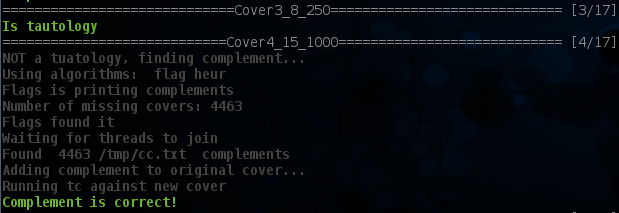
\includegraphics[height=1.6in]{./test.png}
\end{figure}

\newpage
\section{Results}

    The tables below summerize the results and performance of our tautology and
    complement checkers for each of the given benchmarks. The `Flags Memory'
    column shows the heap allocation for the flags array. This is computed
    manually as it is static and based off the number of variables per cube.
    The `Heuristic Memory' column shows the maximum size our algorithm
    allocated from the heap at once.  This was obtained by using our built in
    memory profiler, which wraps malloc and free and logs all allocations and
    decallocations to a file. We then looked for time in our execution where our
    memory was the highest. The `Reported RSS Memory' is the memory usage as
    reported by the standard Linux tools like \texttt{time}, \texttt{ps}, or
    \texttt{top}. The RSS memory is actually slightly decieving as it also
    includes shared memory. The `Faster Algorithm' column indicates which
    algorithm found the answer and finished first.

    \subsubsection{TC Performance}

    We can see from the table below that the flags algorithm seems to always be
    faster at identifying covers that are tautologies, with the exception of
    the really smaller cover files where the difference in time between the two
    algorithms is negligable. We can also see that our memory usage seems to
    climb pretty high for our heuristic algorithm. Looking at the profile plots
    on the following pages we can see that for some covers (like Cover 5 and 8) there
    appears to be a memory leak. Unfortunately we were unable to identifiy it.

    \begin{table}[H]
        \centering
        \begin{tabular}{l|c|r|r|r|r|c}
            \toprule
            \specialcell{Benchmark} &
            \specialcell{Tautology} &
            \specialcell{Execution\\Time(s)} &
            \specialcell{Flags\\Memory} &
            \specialcell{Heuristic\\Memory} &
            \specialcell{Reported\\RSS Memory} &
            \specialcell{Faster\\Algorithm} \\
            \midrule
            Cover1\_8\_10        & NO  & 0.00     & 32B   & -         & 3.360MB   & Heuristic \\
            Cover2\_8\_100       & NO  & 0.00     & 32B   & 9KB       & 3.472MB   & Flags \\
            Cover3\_8\_250       & YES & 0.02     & 32B   & 22KB      & 3.808MB   & Flags \\
            Cover4\_15\_1000     & NO  & 0.00     & 4KB   & 124KB     & 4.704MB   & Heuristic\\
            Cover5\_15\_10000    & YES & 0.24     & 4KB   & 1.449MB   & 14.928MB  & Flags \\
            Cover6\_15\_30000    & YES & 0.01     & 4KB   & 4.084MB   & 34.080MB  & Flags \\
            Cover7\_20\_10000    & NO  & 0.05     & 131KB & 1.513MB   & 10.816MB  & Heuristic\\
            Cover8\_20\_100000   & YES & 21.69    & 131KB & 21.458MB  & 135.968MB & Flags\\
            Cover9\_20\_1000000  & YES & 13.54    & 131KB & 164.462MB & 1.025GB   & Flags \\
            Cover\_25\_100000    & NO  & 0.58     & 4MB   & 18.207MB  & 124.608MB & Heuristic \\
            Cover\_25\_1000000   & YES & 449.00   & 4MB   & 226.092MB & 1.320GB   & Flags \\
            Cover\_25\_10000000  & YES & 480.58   & 4MB   & 1.971GB   & 11.559GB  & Flags \\
            Cover\_30\_1000000   & NO  & 9.38     & 134MB & 210.996MB & 1.805GB   & Heuristic \\
            Cover\_30\_10000000  & YES & 17981.09 & 134MB & 2.636GB   & 16.566GB  & Flags\\
            Cover\_30\_100000000 & YES & 18656.40 & 134MB & 14.552GB  & 125.263GB & Flags\\
            \bottomrule
        \end{tabular}
    \end{table}

    \subsubsection{CC Performance}

    From the table below we can see that the flags algorithm dominates when it
    comes to finding the missing covers fast. Like our \texttt{tc} program
    there appears to be a memory leak that manifiests in some covers like Cover
    4. Other covers, such as Cover 5 do not seem to cause leaks. We were unable
    to pinpoint where we were losing this memory.

    \begin{table}[H]
        \centering
        \begin{tabular}{l|r|r|r|r|c}
            \toprule
            \specialcell{Benchmark} &
            \specialcell{Execution\\Time(s)} &
            \specialcell{Flags\\Memory} &
            \specialcell{Heuristic\\Memory} &
            \specialcell{Reported\\RSS Memory} &
            \specialcell{Faster\\Algorithm} \\
            \midrule
            Cover1\_8\_10        & 0.00     & 32B   & 1.656KB   & 3.680MB   & Flags \\
            Cover2\_8\_100       & 0.00     & 32B   & 6.679KB   & 3.808MB   & Flags \\
            Cover3\_8\_250       & 0.02     & 32B   & 15.789KB  & 3.504MB   & Flags \\
            Cover4\_15\_1000     & 0.11     & 4KB   & 120.775KB & 4.640MB   & Flags \\
            Cover5\_15\_10000    & 0.23     & 4KB   & 899.670KB & 9.904MB   & Flags \\
            Cover6\_15\_30000    & 0.28     & 4KB   & 2.682MB   & 22.464MB  & Flags \\
            Cover7\_20\_10000    & 4.08     & 131KB & 577.593KB & 13.536MB  & Flags \\
            Cover8\_20\_100000   & 11.20    & 131KB & 10.938MB  & 66.592MB  & Flags \\
            Cover9\_20\_1000000  & 13.66    & 131KB & 109.235MB & 626.864MB & Flags \\
            Cover\_25\_100000    & 161.77   & 4MB   & 21.771MB  & 168.016MB & Flags \\
            Cover\_25\_1000000   & 452.42   & 4MB   & 128.959MB & 895.152MB & Flags \\
            Cover\_25\_10000000  & 480.53   & 4MB   & 1.288GB   & 8.765GB   & Flags \\
            Cover\_30\_1000000   & 6269.12  & 134MB & 305.227MB & 2.324GB   & Flags \\
            Cover\_30\_10000000  & 18074.69 & 134MB & 1.484GB   & 9.277GB   & Flags \\
            Cover\_30\_100000000 & 19045.47 & 134MB & 6.454GB   & 88.025GB  & Flags \\
            \bottomrule
        \end{tabular}
    \end{table}

    \newpage
    \putplot{Cover1\_8\_10}{../benchmarks/Cover1_8_10_log_tc.png}{../benchmarks/Cover1_8_10_log_cc.png}
    \putplot{Cover2\_8\_100}{../benchmarks/Cover2_8_100_log_tc.png}{../benchmarks/Cover2_8_100_log_cc.png}
    \putplot{Cover3\_8\_250}{../benchmarks/Cover3_8_250_log_tc.png}{./blank.png}
    \putplot{Cover4\_15\_1000}{../benchmarks/Cover4_15_1000_log_tc.png}{../benchmarks/Cover4_15_1000_log_cc.png}
    \putplot{Cover5\_15\_10000}{../benchmarks/Cover5_15_10000_log_tc.png}{../benchmarks/Cover5_15_10000_log_cc.png}
    \putplot{Cover6\_15\_30000}{../benchmarks/Cover6_15_30000_log_tc.png}{../benchmarks/Cover6_15_30000_log_cc.png}
    \putplot{Cover7\_20\_10000}{../benchmarks/Cover7_20_10000_log_tc.png}{../benchmarks/Cover7_20_10000_log_cc.png}
    \putplot{Cover8\_20\_100000}{../benchmarks/Cover8_20_100000_log_tc.png}{../benchmarks/Cover8_20_100000_log_cc.png}
    \putplot{Cover9\_20\_1000000}{../benchmarks/Cover9_20_1000000_log_tc.png}{../benchmarks/Cover9_20_1000000_log_cc.png}
    \putplot{Cover\_25\_100000}{../benchmarks/Cover_25_100000_log_tc.png}{../benchmarks/Cover_25_100000_log_cc.png}
    \putplot{Cover\_25\_1000000}{../benchmarks/Cover_25_1000000_log_tc.png}{../benchmarks/Cover_25_1000000_log_cc.png}
    \putplot{Cover\_25\_10000000}{../benchmarks/Cover_25_10000000_log_tc.png}{../benchmarks/Cover_25_10000000_log_cc.png}
    \putplot{Cover\_30\_1000000}{../benchmarks/Cover_30_1000000_log_tc.png}{../benchmarks/Cover_30_1000000_log_cc.png}
    \putplot{Cover\_30\_10000000}{../benchmarks/Cover_30_10000000_log_tc.png}{../benchmarks/Cover_30_10000000_log_cc.png}
    \putplot{Cover\_30\_100000000}{../benchmarks/Cover_30_100000000_log_tc.png}{../benchmarks/Cover_30_100000000_log_cc.png}

%Include a retrospective describing what you think is the cause of the good/poor performance of your
%tools and how might you be able to improve the performance if you had more time?

\newpage
\section{Retrospective}
Overall we feel that our results are acceptable. We can run all but the two
biggest \texttt{Cover\_30} in acceptable time and system requirements. Having
the flags algorithm run in parallel provided a really nice speed boost and the
simplicity of it (only 170 lines!) makes it a no brainer to implement. We think
it would be interesting to extend the idea of parallelism into the heuristic
algorithm since in both \texttt{tc} and \texttt{cc} we pretty much split the
matrix in two right away.

There are definitely improvements to be made in our implementation. For one,
there seems to still be some memory leaks in both our programs. We were able to
use \texttt{valgrind} to find and fix a lot of leaks but there are still a few
that remain. Looking at the profile plots in the above section you can clearly
see an upward trend in memory even though the recursion depth is not
increasing, CC Cover 7 is a good illustration of this. Additionally, we spend a
lot of CPU cycles re-finding the most unate and binate columns. A better
strategy would be to only search for them once at the beginning and then just
recalculate where the they are every time we modify the matrix instead of
re-searching.

In the end we were able to successfully run all the provided benchmarks and our
\texttt{test.sh} script proves that we can take a non tautology cover, find the
complements, put those complements back into the original cover, and then prove
that it is now a tautology. Given this fact we are confident in saying our
implementation was successful.



\end{document}
